\documentclass[a4paper,12pt]{extarticle}
\usepackage[top=3cm]{geometry}

\usepackage{titling}
\setlength{\droptitle}{12em}

\usepackage[scaled]{helvet}
\renewcommand\familydefault{\sfdefault} 
\usepackage[T1]{fontenc}
\usepackage{graphicx}
\usepackage{hyperref}

\usepackage[usenames, dvipsnames]{color}
\definecolor{mygray}{rgb}{0.5, 0.5, 0.5}
\definecolor{mygreen}{rgb}{0,0.6,0}
\definecolor{myblue}{RGB}{57, 135, 189}

\usepackage{listings}
\lstset{ 
    language=java,
    basicstyle=\ttfamily\footnotesize,
    keywordstyle=\color{myblue},
    commentstyle=\color{mygray},
    stringstyle=\color{mygreen},
    frame=single,
    showstringspaces=false,
}

\title{\textbf{Software Engineering\\\vspace{5mm} CPS2002\\\vspace{5mm}  Assignment Report}}

\author{\LARGE Martin Bartolo - 0218300L\vspace{1mm}\\ \LARGE Mikhail Cassar - 0319599M\vspace{3mm}\\ \large BSc (Hons) Computing Science and Mathematics}

\date{Assignment due 27\textsuperscript{th} May 2019}

\setcounter{secnumdepth}{0}

\begin{document}

\setlength{\parindent}{10pt}
\setlength{\footskip}{50pt}
\pagenumbering{arabic}

\maketitle
\thispagestyle{empty}
\newpage

\tableofcontents
\newpage

\section{Introduction}
The aim of this assignment was to collaboratively work on a software project, with the main focus being on rigorous software testing and the use of Git. Our first task was to set up our environments, namely our Git repository on Github and our Jenkins environment on the University Jenkins server. First, we initialised our Git repository and ensured that each team member could commit changes and push and pull them from Github. When this was ensured, we set up our Jenkins environment to work with Maven and scan for changes from Github every few minutes. Whenever changes are found, they are built and run with a detailed code coverage report and test results being displayed using the Emma plug-in. Our progress at this point can be seen by viewing the "Part1" tag on our Github repository. After completing our set-up, we were ready to start working on the two remaining tasks which will be discussed in detail throughout the remainder of this report.
\newpage

\section{InitialGame Design}
\noindent The design of the game consists of sectioning the game into different classes, here we will talk about the contents of those classes while also explain how they all work together.\\

\noindent The information provided will be regarding the basic version of the game i.e. before any enhancements to the game were made. The basic version of the game is found in the tag "Part2".

\subsubsection{Game Class}

\noindent The \textit{Game} class contains the most essential parts of the game, this is because it encompasses all the other parts of the game. Also this class contains the \textit{Main} class and so this is where the game executes. Below is a listing showing the main game loop.

\begin{lstlisting}
 public static void main(String[] args) {
        //This variable is used to hold the 
        //previous directions taken by a given player
        String directions;

        System.out.print("Welcome to the Treasure Map Game by Martin 
        Bartolo and Mikhail Cassar");
        Game game = new Game();

        //Run startGame method to initialise players and map
        game.startGame(game);
        
	// will be set to true when the treasure
        //is found by one of the players
        boolean foundTreasure = false;
        
        //An array which holds all the players 
        //who found the treasure on a given turn
        //This is just in case more than one 
        //player finds it on the same turn
        boolean[] winners = new boolean[game.players.size()];

        //Generating the initial html files here before 
        //there are any moves
        //Generating an html file for each player in the game
        for(int i = 0; i < game.players.size(); i++){

         if(game.generateHtmlFile(i, game.map.mapSize, " ") == 0){
             System.err.println("Could not generate HTML files");
         }
        }

        //Main game loop
        while (true) {
        
        //Increment amount of turns 
        //which have been played        
            game.turns++;

            System.out.println("-------------------------------\n");

            //Get each players desired direction 
            //of movement for the current turn
            game.directionsLoop();

            //Generating an html file for each 
            //player's current state
            for(int i = 0; i < game.players.size(); i++){

                //Obtaining the last 4 directions of each player
                directions = game.getPreviousDirections(i);

                if(game.generateHtmlFile(i, game.map.mapSize
                ,directions) == 0){
                    System.err.println("Could not generate 
                    HTML files");
                }
            }

            //Go through each player in the 
            //game and check if they found the treasure
            //Mark the players who have found the treasure
            int i = 0;
            for(Player player: game.players){

                if(player.foundTreasure){
                    foundTreasure = true;
                    winners[i] = true;
                }
                i++;
            }

            //If the treasure has been found by one of the players
            if (foundTreasure) {

                for(i = 0; i < winners.length; i++){

                    if (winners[i]){
                        System.out.println("Congratualtions player "
                         + (i+1) + ", you have found the treasure
                          in " + game.turns + " turns!");
                    }
                }
                break;
            }
        }

        System.out.println("---------------------------------\n");

        //After a player wins the game the user is able to
        //prompted to exit the game
        game.exitGame(game);
    }

    //Method to initialise map along with players and
    // their starting positions
    private void startGame(Game game) {
        game.playerNum = getPlayerNum();

        map.mapSize = getMapSize();
        map.generate();// Generate map

        //In this loop all the Player objects are created 
        //along with their starting position in the map
        for (int i = 0; i < game.playerNum; i++) {

            //A new player object is made
            Player player = new Player();

            //The random position of the player is 
            //set to a grass tile
            player.position = player.setStartingPosition(
            map.getGrassTiles());

            //The created player is added to the ArrayList of players
            players.add(player);
        }
    }

\end{lstlisting}
\vspace{4mm}

\noindent The design of the \textit{Game} class needed to include an efficient method on how to organise the implementation of the \textit{Player} objects and the \textit{Map} object. All of this processing is first done in the \textit{startGame()} Method, since this is where the initialisation and setting up of the game takes place.\\

\newpage
\begin{lstlisting}
  //Method to initialise map along with players and
    // their starting positions
    private void startGame(Game game) {
        game.playerNum = getPlayerNum();

        map.mapSize = getMapSize();
        map.generate();// Generate map

        //In this loop all the Player objects are created 
        //along with their starting position in the map
        for (int i = 0; i < game.playerNum; i++) {

            //A new player object is made
            Player player = new Player();

            //The random position of the player is 
            //set to a grass tile
            player.position = 
            player.setStartingPosition(map.getGrassTiles());

            //The created player is added to the ArrayList of players
            players.add(player);
        }
    }
\end{lstlisting}
\vspace{4mm}

\noindent This method is called in the beginning of the \textit{Main} class. The number of players and the map size is obtained from the user initially and with that information the game can be set up. First the \textit{Map} object created will have a tile map generated for it. This is taken care of in the \textit{generate()} method in the \textit{Map} class.\\

\begin{center}
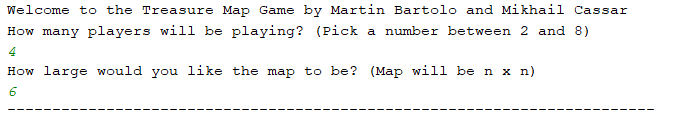
\includegraphics[scale=0.5]{BasicMap2.png}\\
Asking the player to input the number of players and the size of the map
\end{center}

\noindent After generating the tile map, the \textit{Player} objects are created, initialised (by being given a starting position) and placed into an array list. By doing this the \textit{Player} objects are easier to handle.\\

\noindent After setting up the game and thus exiting the \textit{startGame()} method, an initial map file is generated for each player using the\textit{generateHtmlFile} method in the \textit{main} method. This method generates an html file for each player with all the tiles being gray except the tiles which the current player has landed on.\\

\newpage
\begin{lstlisting}
  //Method to initialise map along with players and
    // their starting positions
    private void startGame(Game game) {
        game.playerNum = getPlayerNum();

        map.mapSize = getMapSize();
        map.generate();// Generate map

        //In this loop all the Player objects are created 
        //along with their starting position in the map
        for (int i = 0; i < game.playerNum; i++) {

            //A new player object is made
            Player player = new Player();

            //The random position of the player is 
            //set to a grass tile
            player.position = 
            player.setStartingPosition(map.getGrassTiles());

            //The created player is added to the ArrayList of players
            players.add(player);
        }
    }
\end{lstlisting}
\vspace{4mm}

\noindent During the actual game the same \textit{generateHtmlFile()} method is used when generating the files at the HTML files at the end of turn , however here the full functionality of the method is used, the previous directions and the previous positions of the current player are displayed in the HTML file. Given there are various tile types within the game, a conditional statement is used within the \textit{generateHtmlFile()} method which displays the corresponding colour depending on the tile type. The code mentioned is displayed below.

\begin{lstlisting}

switch(tileType){
                    //Grass tile
                    case 0:

                        if(playerHere){

                            htmlText.append("<div class=\
                            "cellGreen\">" +
                                    "<img src=\
                                    "player.png\" alt=
                                    \"player\">" +
                                    "</div>\n");
                        }

                        else{

                            htmlText.append("<div class=\
                            "cellGreen\"></div>\n");

                        }
                        break;

                    //Water tile
                    case 1:

                        if(playerHere){

                            htmlText.append("<div class=\
                            "cellBlue\">" +
                                    "<img src=\
                                    "player.png\" alt=\
                                    "player\">" +
                                    "</div>\n");
                        }

                        else{

                            htmlText.append("<div class=\
                            "cellBlue\"></div>\n");

                        }
                        break;

                    //Treasure Tile
                    case 2:

                        if(playerHere){

                            htmlText.append("<div class=\
                            "cellYellow\">" +
                                    "<img src=\
                                    "player.png\" alt=\
                                    "player\">" +
                                    "</div>\n");

                        }

                        else{

                            htmlText.append("<div class=\
                            "cellYellow\"></div>\n");

                        }
                        break;

                    default:
                        //No need to check for player here
                        //as a player can never be on a gray tile
                        htmlText.append("<div class=\
                        "cellGray\"></div>\n");
                        break;
                }
            }

\end{lstlisting}
\vspace{4mm}

\newpage
\noindent After setting up the map files, the game starts. A loop is made which keeps on iterating until a player wins, each \textit{Player} object has a check which is raised if the player lands on the winning tile.\\

During each turn of the game, each player is asked to input a direction depending on where they want to move. The \textit{directionsLoop} method manages this.\\

\begin{lstlisting}

//Loop through each player in ArrayList
        for (Player player : players) {
            System.out.println("Player " + (players.indexOf(player) 
            + 1) + ", please choose a direction (u, d, l or r).");

            validMove = false;
            while (!validMove) {
                direction = 'x';
                //Make sure that user input is
                //valid (i.e. one of u, d, l or r)
                while(direction == 'x' || direction == 'y') {
                    scanner = new Scanner(System.in);
                    direction = validateDirectionInput(scanner);
                }

                //Check if move is within map and execute if it is
                if (checkOutOfBounds(direction, player, map.mapSize)
                 == 1) {
                    validMove = true;

                    //Change player's position variables 
                    //to new position
                    player.move(direction);

                    //Triggers event for corresponding tile type
                    map.evaluateCurrentPlayerTile(player);
                }
            }
        }

\end{lstlisting}
\vspace{4mm}

\noindent As mentioned before the HTML file for each player is updated at the end of each turn, also at the end of each turn the treasure flag of each player is checked to determine if a player has landed on the treasure tile. If at least one player has stepped on the treasure tile, the game stops at the end of the turn and the winners are displayed.\\

\noindent All user input within the game is taken care of by validation methods, so if the user gives incorrect input the program will not crash.\\
\newpage
\subsubsection{Map Class}
\noindent The \textit{Map} class is used to generate the tile map structure which the game is played on. Apart from that, the tile events which occur are also taken care of by the Map class.\\

\noindent The map generation which occurs in the \textit{startGame()} method basically constructs a 2-dimensional array called \textit{tiles}, which is the size of the map in both dimensions. The array holds the tile type of each tile positions in the game. Each position in the \textit{tiles} array corresponds to a tile in the map. Below one can see how each tile is randomly generated.

\begin{lstlisting}
//Keep on looping until all tiles are randomly generated
        while(generatedTilesNum(generatedTiles) != mapSize*mapSize){

            //Randomly generate a pair of tiles
            //Numbers generated will be from 0 to mapSize-1
            randomPair[0] = random.nextInt(mapSize);
            randomPair[1] = random.nextInt(mapSize);

            //Now checking if the tile has already been obtained 
            //in the generated tiles
            //This is done by checking if the boolean 
            //value of the tile is true
            if(generatedTiles[randomPair[0]][randomPair[1]][0]){
                //Tile has already been generated
                //So the user must get another tile which
                //has not already been generated

                //Keeps on looping until a new tile is generated
                while(generatedTiles[randomPair[0]]
                [randomPair[1]][0]){

                    randomPair[0] = random.nextInt(mapSize);
                    randomPair[1] = random.nextInt(mapSize);

                }
            }
\end{lstlisting}
\vspace{4mm}

\noindent After a tile is randomly generated, a tile type has to be assigned, this is done using the below code within the same \textit{generate()} method. The tile type is an integer from 0 to 2, since there are three types in the current implementation of the game, however if a new tile wants to be included in the game, this can easily be done with this implementation. Below is the code of how the tile types are assigned to a given tile position.

\begin{center}

\includegraphics[scale=1]{greyTile.png}
\hspace{1mm}

\includegraphics[scale=1]{greenTile.png}
\hspace{1mm}

\includegraphics[scale=1]{blueTile.png}
\hspace{1mm}

\includegraphics[scale=1]{yellowTile.png}
\hspace{1mm}

Each tile implemented within the game
\end{center}

\newpage
\begin{lstlisting}

 //Keep on looping until the current tile is given a tile type
            do {

                //Set the tile type for the newly generated tile
                //A random number from 0 to 2 is obtained which 
                //correspond to a tile type
                tileType = random.nextInt(3);

                //A switch statement is used to go through
                //each of the possible tile types
                switch (tileType) {

                    //Grass tile
                    case 0:
                        tiles[randomPair[0]][randomPair[1]][0] = 0;

                        //The counter is updated since another 
                        //grass tile has been added to the map
                        grassCount += 1;

                        break;

                    //Water tile
                    case 1:
                        if (waterCount == waterMaxTiles) {
                            //When the maximum number of water 
                            //tiles is reached the check 
                            //is set to true
                            //This is so that the while loop 
                            //will continue until a random 
                            //number is obtained which
                            //is not full
                            continue;

                        } else {
                            tiles[randomPair[0]][randomPair[1]][0] 
                            = 1;

                            //The counter is updated since another 
                            //water tile has been added to the map
                            waterCount += 1;
                        }
                        break;

                    //Treasure tile
                    case 2:

                        if (treasureCount == treasureMaxTiles) {
                            //When a treasure tile is already placed 
                            //the check is set to true
                            continue;
                        } else {
                            tiles[randomPair[0]][randomPair[1]][0]
                             = 2;
                            //The counter is updated since a teasure
                            // tile has been added to the map
                            treasureCount += 1;
                        }
                        break;

                    default:
                        //This case is accessed only when a random 
                        //number which is not 0,1 or 2 is obtained
                        System.err.println("Invalid random 
                        number obtained");
                        break;
                
\end{lstlisting}
\vspace{4mm}

\newpage
\subsubsection{Player Class}
\noindent The Player class manages the individual properties of a player, such as the tile positions and the directions the player has traversed.\\

\noindent When a \textit{Player} object is created the positions and the directions the \textit{Player} has moved are saved using an array list for each.

\begin{lstlisting}
  //This array list is used to hold the previous 
  //positions the player
    ArrayList<Position> positions = new ArrayList<Position>();

  //This array list is used to hold the previous directions#
  //of the player
    ArrayList<String> directions = new ArrayList<String>();
\end{lstlisting}
\vspace{4mm}

\noindent In the \textit{startGame()} method, a starting position is set for each new \textit{Player} object which is created, this is done using the \textit{setStartingPosition()} method, this method takes two random values from a \textit{grassTiles} array, which holds all the tile positions of grass tiles within the tile map, these two numbers are added to the \textit{positions} array list of the player and the player is displayed starting at this position.

\begin{lstlisting}
    //This method sets the starting position of a player
    Position setStartingPosition(int[][] grassTiles){

        Random random = new Random();

        Position position = new Position(0, 0);

        //Obtaining the length of grassTiles so as to be able to 
        //know from which range to obtain a random number
        int grassCount = grassTiles.length;

        //random number from 0 to length of grassTiles is obtained
        int grassTilesIndex = random.nextInt(grassCount);

        //The start position is set
        position.x = grassTiles[grassTilesIndex][0];
        position.y = grassTiles[grassTilesIndex][1];

        //The current position of the player is set 
        //to the start position
        this.position = position;

        //The start positions is added to the created player
        addToPositions(position.x, position.y);

        return position;
    }
\end{lstlisting}
\vspace{4mm}

\newpage
\noindent This class also modifies the current position of the current player through the use of the \textit{move()}. Depending on which direction the player moves, the current position of the player is modified and the added to the \textit{positions} array list, the given direction is added to the \textit{directions} array list.

\begin{lstlisting}

//Method to move the player's position according to a 
//given direction
    void move(char direction){

        //A switch statement is used to represent all 
        //possible directions
        switch(direction){
            case 'l':
                // change player's position
                this.position.x --;
                // add position to list of previous positions
                addToPositions(position.x, position.y);
                // add direction to list of previous directions
                directions.add("left");
                break;

            case 'r':
                // change player's position
                this.position.x ++;
                // add position to list of previous positions
                addToPositions(position.x, position.y);
                // add direction to list of previous directions
                directions.add("right");
                break;

            case 'u':
                // change player's position
                this.position.y --;
                // add position to list of previous positions
                addToPositions(position.x, position.y);
                // add direction to list of previous directions
                directions.add("up");
                break;

            case 'd':
                // change player's position
                this.position.y ++;
                // add position to list of previous positions
                addToPositions(position.x, position.y);
                // add direction to list of previous directions
                directions.add("down");
                break;

            default:
                break;
        }
    }

\end{lstlisting}
\vspace{4mm}

\newpage

\begin{center}
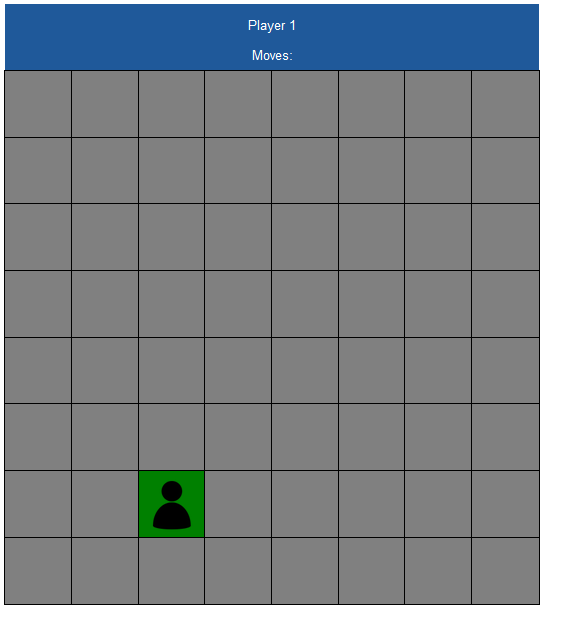
\includegraphics[width=\textwidth]{BasicMap1.png}\\
The initial position of a player when the game starts
\end{center}

\newpage
\subsubsection{Position Class}

The \textit{Position} class is used to simplify the way in which the program interprets the player's location within the tile map.\\

\noindent As seen in the class diagram, a \textit{Position} class is used by \textit{Player} objects, so any instacnes of \textit{Position} objects are within the \textit{Player} objects.

\begin{lstlisting}
public class Position {

    //Value of each coordinate
    int x;
    int y;

    //Method to display a position object
    @Override
    public String toString() {
        return "Position{" +
                "x=" + x +
                ", y=" + y +
                '}';
    }

    //Constructor for the player object
    Position(){
    }

    //Constructor for the position object when both 
    //x and y values are given
    Position(int px, int py) {
        x = px;
        y = py;
}
\end{lstlisting}
\vspace{4mm}

\newpage
\section{Enhancements}
\subsection{Different Map Types}

The design pattern chosen for this enhancement was the \textbf{factory design pattern}. Since this enhancement was centred around the map's creation then it was clear that a creational design pattern had to be chosen. The main things which needed to be kept in mind were that 2 initial map types had to be implemented while more map types could easily be added to the future. Therefore, the Factory design pattern was the most suitable for the task.\\

The class diagram of the enhancement can be seen below.\\

\begin{center}
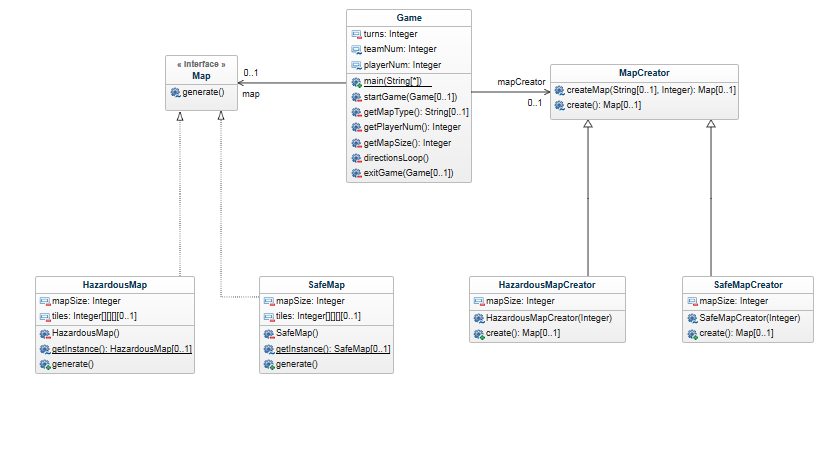
\includegraphics[width=\textwidth]{Enhancement1CD.png}\\
\end{center}

\newpage

\noindent Our implementation is centred around a \textit{Map} interface which contains each method which will be used by the different map types. Each type of map then has a class which implements this main \textit{Map} interface as can be seen in the class diagram above. This design allows for the easy implementation of additional map types in the future.\par

A factory method is present in the \textit{MapCreator} class which is passed the map's type and its size. This class has a creator subclass for every map type, allowing for easy creation of additional map types in the future. An instance of the correct creator subclass will then be made and used to create the map. This can be seen in the code snippet below.

\vspace{-1mm}
\begin{lstlisting}
//Factory Method
Map createMap(String type, int mapSize){

    MapCreator creator;

    if(type.equals("safe")){
        creator = new SafeMapCreator(mapSize);
    }
    else if(type.equals("hazardous")){
        creator = new HazardousMapCreator(mapSize);
    }
    else{
        creator = null;
        System.err.println("Invalid map type");
    }

    if (creator != null) {
        return creator.create();
    }
    else{
        return null;
    }
}
\end{lstlisting}
\vspace{4mm}

\noindent The map is then created in the appropriate creator subclass by setting the map size and calling the generate method in the map type's class (either the \textit{SafeMap} or \textit{HazardousMap} class in our implementation but more can easily be added). A code snippet of this create method for the "safe" map type is shown below

\vspace{-1mm}
\begin{lstlisting}
//Method to create and return a safe map
@Override
public Map create(){
    //getInstance method used here to obtain a 
    //static instance of the hazardous map
    SafeMap map =  SafeMap.getInstance();
    map.setMapSize(mapSize);
    map.generate();
    return map;
}
\end{lstlisting}

\noindent In the generate method for the safe map, the maximum amount of water tiles is set to 10\% and then rounded down to the nearest integer. This code snippet is shown below.

\begin{lstlisting}
//The maximum number of water tiles in a map is set to
//10% of the total tiles
int waterMaxTiles = (int) Math.floor((mapSize*mapSize) * 0.1);
\end{lstlisting}
\vspace{4mm}

\noindent In the generate method for the hazardous map, the maximum amount of water tiles is set to 25\% and then rounded up to the nearest integer. This code snippet is shown below.

\begin{lstlisting}
//The maximum number of water tiles in a map is set to 
//25% of the total tiles
int waterMaxTiles = (int) Math.ceil((mapSize*mapSize) * 0.25);
\end{lstlisting}
\vspace{4mm}

\noindent Apart than these changes, the map is generated as it was in the generate method in the basic version of the program before the enhancements.\\

\noindent When running the program, the user is asked what map type they would like to play with. This can be seen below.

\begin{center}
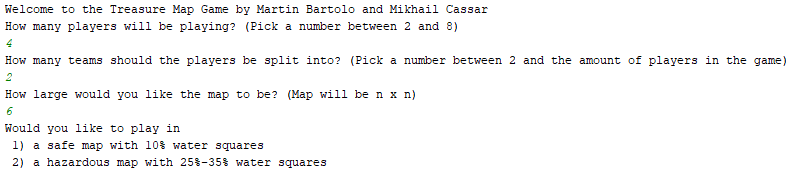
\includegraphics[width=\textwidth]{Figure1.png}
\end{center}

\noindent After the user chooses the map type, the map is created as discussed on the previous page and then the game can be played. On the next page is a comparison between the ending screen of a game played by 4 players in 2 teams on a 6x6 safe map and a game played by the same players on a 6x6 hazardous map. Notice the different amounts of water tiles encountered between the 2 map types.
\newpage

\begin{center}
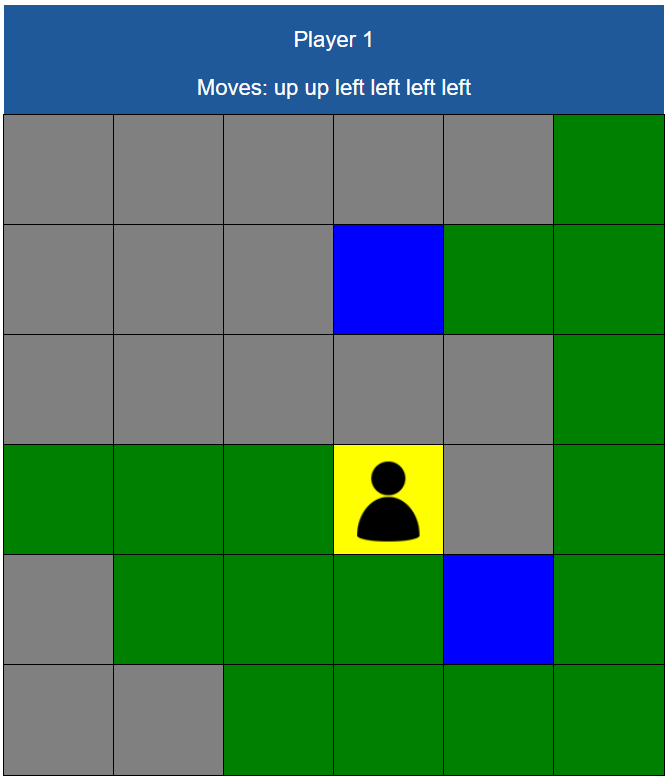
\includegraphics[scale=0.5]{Figure2.png}\\
Ending screen of game using a safe map
\end{center}

\begin{center}
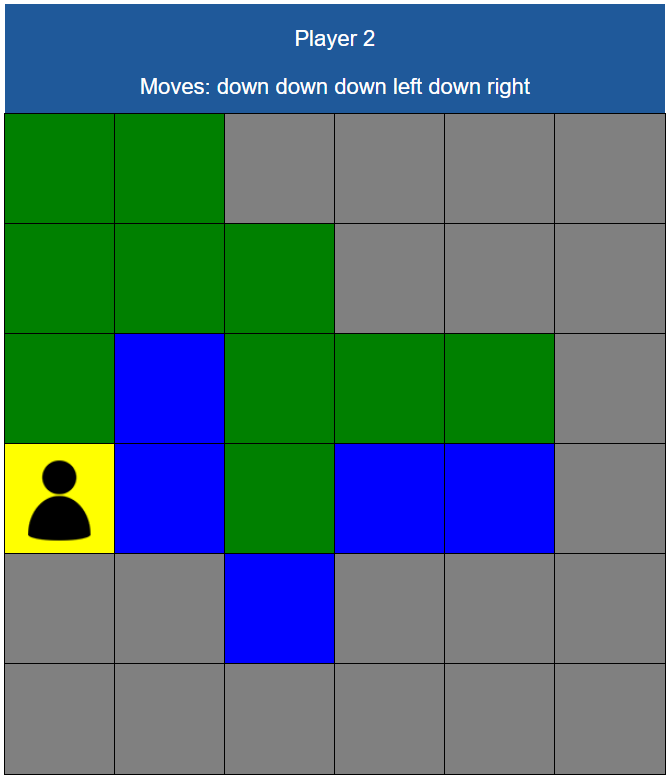
\includegraphics[scale=0.5]{Figure3.png}\\
Ending screen of game using a hazardous map
\end{center}

\newpage

\subsection{Single Map File}

The design pattern chosen for this enhancement was the \textbf{singleton design pattern}. Since the problem involved the creation of only one map file it was clear that a creational design pattern was needed. The problem which needed to be solved here was that there was only one instance of a map file throughout the whole game. This could easily be taken care of using the Singleton design pattern.\\

\noindent The class diagram of the enhancement can be seen below.\\

\begin{center}
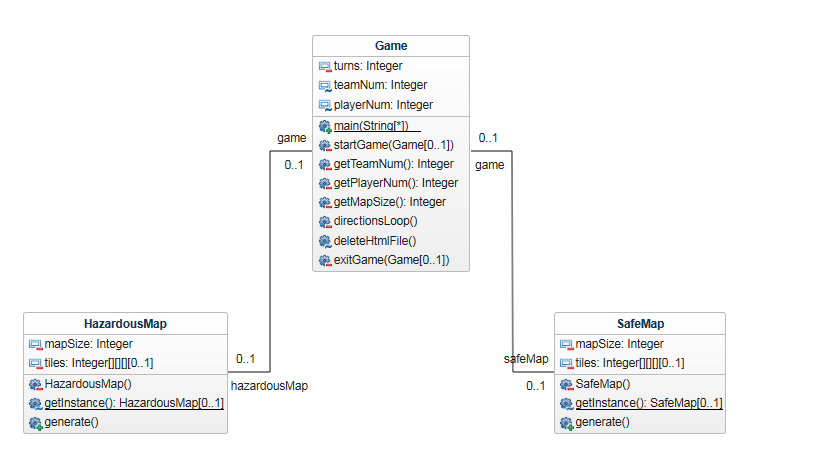
\includegraphics[width=\textwidth]{Enhancement2CD.png}\\
\end{center}

\noindent Given the first enhancement led to the creation of the \textit{safeMap} class and \textit{hazardousMap} class, a singleton design patter for each subclass has to be implemented since they produce different objects.\\

\noindent After the user chooses which map type they want, through the process previously defined in the first enhancement, the program goes to the corresponding \textit{Map} subclass through the \textit{MapCreator} class.\\ 

\noindent In the \textit{SafeMap} class and \textit{HazardousMap} class, a private static instance is initialised. By doing this the \textit{Map} object cannot be used in any other method and since it is static the object will be directly affected at every change which occurs throughout the lifetime of the program. This means that given only one map, and hence one map file, any change which occurs will affect that single map file and so there is only one map file which is being affected. This can be seen in the screenshot below.\\


\begin{center}
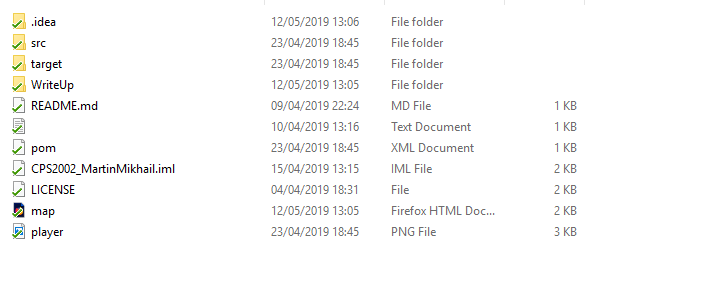
\includegraphics[width=\textwidth]{Singleton1.png}\\
Local repository containing a single map file
\end{center}


\noindent A \textit{getInstance()} method is also created in the subclasses. This method declares the previously initialised static object created. However, the object is declared only if the object is null. This is so because it would lead to the creation of a new object and so this method takes care of that.\\

\newpage
\begin{lstlisting}

    private static SafeMap map = null;

    //Constructor for SafeMap
    private SafeMap(){
    }

    //This method is used to obtain the static 
    //instance of the object
    static SafeMap getInstance(){
            if(map == null){
                map = new SafeMap();
            }

            return map;
    }
    
\end{lstlisting}
\vspace{4mm}


\begin{lstlisting}
 //A static instance is created to implement the 
 //singleton design pattern
    private static HazardousMap map = null;

    //constructor for HazardousMap
    //Constructor is set to private to implement the 
    //singleton design pattern
    private HazardousMap(){
    }

    //This method is used to obtain the static 
    //instance of the object
    static HazardousMap getInstance(){
        if(map == null){
            map = new HazardousMap();
        }

        return map;
    }

\end{lstlisting}
\vspace{4mm}

\noindent In the \textit{CreateMap} class, the \textit{getInstance()} method is used so as to create \textit{Map} object. This is the same for each map type. Hence now after going through this a map object is created which is able to be used by the game.

\newpage
\begin{lstlisting}

 //Method to create and return a safe map
    @Override
    public Map create(){
        //getInstance method used here to obtain
        // a static instance of the hazardous map
        SafeMap map =  SafeMap.getInstance();
        map.setMapSize(mapSize);
        map.generate();
        return map;
    }


\end{lstlisting}
\vspace{4mm}



\begin{lstlisting}

   //Method to create and return a hazardous map
    @Override
    public Map create(){

        //getInstance method used here to obtain 
        //a static instance of the hazardous map
        HazardousMap map = HazardousMap.getInstance();
        map.setMapSize(mapSize);
        map.generate();
        return map;
    }


\end{lstlisting}
\vspace{4mm}

\noindent In the initial idea of the game, a map file was created for each player and at the end of each turn the map file gets updated using the \textit{changeHtmlFile()} method.

\begin{lstlisting}
//A file object is being created where the name is given 
//depending on the number of the player
        File file = new File("map.html");

        //The actual file is created here
        try {
            //If file already exists set return value
            //to 2 to mark that it is being overwritten
            if(!file.createNewFile()){
                returnValue = 2;
            }
        } catch (IOException e) {
            e.printStackTrace();
            returnValue = 0;//Set return value to error
        }
\end{lstlisting}
\vspace{4mm}

\noindent Now instead we have only one file, and that file is changed to the corresponding player's map tile when it is the player's turn to choose their desired direction.

\begin{lstlisting}
 
        //Loop through each player in ArrayList
        for (Player player : players) {

            if(!foundTreasure) {
                //At the end of the current player's turn 
                //the main html file is changed
                teams.get(getTeamIndex(player)).changeHtmlFile
                (players.indexOf(player), map, player);
            }

            System.out.println("Player " + 
            (players.indexOf(player) + 1) +
             ", please choose a direction (u, d, l or r).");
\end{lstlisting}

\newpage
\subsection{Teams}
The design pattern chosen for this enhancement was the \textbf{composite design pattern}. This enhancement required us to rethink the Player concept of the game. We needed to find a way how to add players randomly to a team, this problem was a structural one since this problem deals with the composition of different classes.\\

\begin{center}
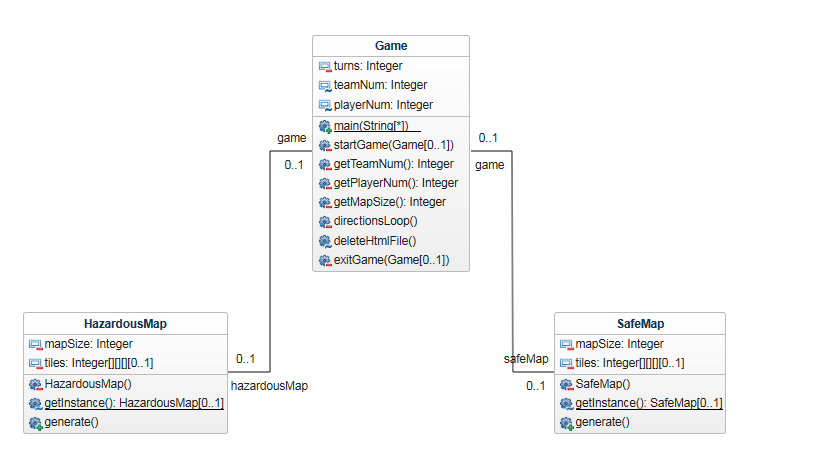
\includegraphics[scale=0.5]{Enhancement2CD.png}\\
Ending screen of game using a hazardous map
\end{center}

\noindent The reason the composite design pattern was a good choice is because this design pattern structures classes into two types:

\begin{enumerate}
\item Leaf
\item Composite
\end{enumerate}

\noindent In our case the Player object corresponds to the Leaf while the Team objects  corresponds to the Composite. The reason this works is because a Leaf can be though of as a unit while a composite contains various leaves, this is just like a team having multiple players in it. Thus a team can be seen as a complex object of multiple singular object.\\

\noindent The composite design pattern goes further with this idea as it allows for composite objects to contain other composite objects, however in our case this would not make as much sense since a team containing a team would not really work well in our game. So our design pattern is a basic implementation of the composite design pattern.\\

\noindent A User interface was implemented as the component within the composite design pattern. This interface is implemented by both the \textit{Player} class and the \textit{Team} class as they are both components with the design pattern.\\

\vspace{-1mm}
\begin{lstlisting}
import java.util.ArrayList;

public interface User {
    //The User interface is the component of the 
    //composite design pattern

    ArrayList<Position> positions = new ArrayList<Position>();

    //Method used to add a position to the positions 
    //ArrayList using the x and y values
    void addToPositions(int posx, int posy);
}
\end{lstlisting}
\vspace{4mm}

\noindent Given this is a basic implementation of the composite design pattern, the component element of the design pattern is not as useful here, since the enhancement could easily be implemented by just using the \textit{Team} class. This is the reason for the \textit{User} interface not having as much common objects between the \textit{Player} subclass and the \textit{Team} subclass.\\

\noindent When running the program, the user is asked how many teams they would like to play with. This can be seen below.

\begin{center}
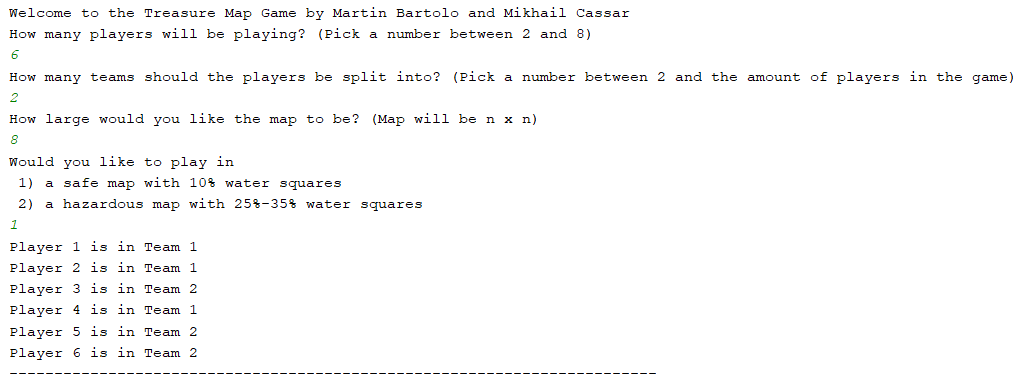
\includegraphics[scale=0.5]{Team3.png}\\
\end{center}

\noindent After the user chooses the number of teams within the game, the players are randomly distributed among the teams. All of this is done within \textit{startGame()} method, using the \textit{generateTeam()} method and the \textit{distributeRemainder()} method.//
\vspace{4mm}

\newpage
\begin{lstlisting}
//Holds the players which have been added to a team
        ArrayList<Player> addedPlayers = new ArrayList<Player>();

        //Now to assign all the player objects to a random team
        for (int i = 0; i < game.teamNum; i++) {

            //A new team is created
            Team team;

            //Generate the team
            team = generateTeam(addedPlayers, playersInTeamNum);

            //Add the team to the list of teams in the game
            teams.add(team);
        }
\end{lstlisting}
\vspace{4mm}

\noindent All the \textit{Player} objects which have already been added to a team are taken into account, this is used so as to add a unique \textit{Player} object to each \textit{Team} object. The random distribution of players is taken care of in the \textit{generateTeam()} method which can be seen below.\\

\begin{lstlisting}
//Method to generate the teams
    Team generateTeam(ArrayList<Player> addedPlayers, 
    int playersInTeamNum){

        Random random = new Random();

        //Check if the current player exists in a team
        boolean playerIsInATeam;

        //Holds a random index of a player
        int rand;

        //A new team is created
        Team team = new Team();

            //Randomly add the specified amount of 
            //players to a team
            //Get playerInTeamNum random players 
            //from the players array list
            for (int j = 0; j < playersInTeamNum; j++) {

                //At each iteration this check is 
                //always initialised to true
                //If there is no matching value in 
                //the array list then the while loop breaks
                playerIsInATeam = false;

                //Keep on looping until a new 
                //player index is obtained
                do {
                    //A random index is obtained
                    rand = random.nextInt(playerNum);

                    //If no player has currently 
                    //been added to a team
                    if(addedPlayers.size() == 0){

                        //A random index is obtained
                        rand = random.nextInt(playerNum);

                        //An initial player has been added
                        team.addPlayer(players.get(rand));

                        addedPlayers.add(players.get(rand));

                        //If the size of a team is only one 
                        //player then this team is full
                        //If not then continue adding players 
                        //until the maximum is reached
                        if(playersInTeamNum== 1){
                            playerIsInATeam = false;
                        }
                    }

                    //If a player has been added to a team
                    else {

                        //Initialised to false since 
                        //we are checking 
                        //if the current player is 
                        //already in a team
                        playerIsInATeam = false;

                        //Loops through all the players which 
                        //are already in a team
                        //Ends when a player which is not in a 
                        //team is obtained
                        for (Player player : addedPlayers) {

                            //If the current player has 
                            //already been generated
                            if (players.get(rand) == player) {
                                playerIsInATeam = true;
                            }
                        }

                        if(!playerIsInATeam){
                            //Add the player to the team
                            team.addPlayer(players.get(rand));

                            addedPlayers.add(players.get(rand));

                            //The check is false and 
                            //the loop is broken
                            break;
                        }
                    }

                    //Keep on looping while the current player 
                    //being obtained is already in a team
                    } while (playerIsInATeam);
            }

        //Returns a team with the player
        return team;
    }
\end{lstlisting}
\vspace{4mm}

\noindent This method works by first creating a \textit{Team} object, and then iterates for the total number of players to add to each team. A random index from the \textit{players} array list is obtained and compared to the indexes of the players within the \textit{addedPlayers} array list. If the random index does not match with any of those in \textit{addedPlayers}, then that player is not in any team and can be added to a team, the player is also added to \textit{addedPlayers}. This is repeated for each team.\\


\noindent At the beginning of each game in the \textit{startGame()} method, after obtaining the number of players and teams, two more values are obtained. The \textit{playersInTeamNum} variable is the total number of players in each team which can all be equally divided into a team. The \textit{extraPlayersNum} is the total number of players which are removed so as to be able to divide the number of players equally at first. 

\newpage
\begin{lstlisting}
        //get number of players from user
        game.playerNum = getPlayerNum();

        //get number of teams from user
        game.teamNum = getTeamNum();

        //The remainder of the total number of players 
        //divided by the total number of teams is obtained
        int extraPlayersNum = playerNum % teamNum;

        //The total number of player per team is obtained 
        //excluding the extra players
        int playersInTeamNum = (playerNum - extraPlayersNum)/teamNum;

\end{lstlisting}
\vspace{4mm}

\noindent The extra players are then randomly inputted into random teams using the \textit{distributeRemainder} method.

\begin{lstlisting}
// Method to distribute the remaining player if 
//the players are not evenly distrubted among the teams
    void distributeRemainder(ArrayList<Player> addedPlayers,
     int extraPlayersNum){

        Random random = new Random();

        //Array list which holds the teams which 
        //have already been generated
        ArrayList<Team> obtainedTeams = new ArrayList<Team>();

        //Check if the current player exists in a team
        boolean playerIsInATeam;

        //check if an extra player is already added to the team
        boolean teamIsFull;

        //Holds a random index for the player 
        //and the team respectively
        int playerIndex;
        int teamIndex;

        //Obtain a player which is not in a team 
        //for extraPlayerNum times
        for(int i = 0; i < extraPlayersNum; i++){

            //First obtain a random unique team
            //This is so only one extra player is added 
            //to a team so there would not be much of 
            //a disadvantage to the other players

            //Keep on looping until a new team index is obtained
            do {

                teamIsFull = false;

                //A random index is obtained
                teamIndex = random.nextInt(teamNum);

                //This is used so as to set up the 
                //obtainedTeams array list
                if(obtainedTeams.size() == 0){

                    obtainedTeams.add(teams.get(teamIndex));

                }

                else{

                    for (Team team : obtainedTeams) {

                        //If the current player has 
                        //already been generated
                        if (teams.get(teamIndex) == team) {
                            teamIsFull = true;
                        }
                    }

                }

            }while(teamIsFull);

            //Now a new team is obtained with every iteration
            //Keep on looping until a new player index is obtained
            do {
                //At each iteration the checks are set to false
                playerIsInATeam = false;

                //A random index is obtained
                playerIndex = random.nextInt(playerNum);

                for (Player player : addedPlayers) {

                    //If the current player has 
                    //already been generated
                    if (players.get(playerIndex) == player) {
                        playerIsInATeam = true;
                    }
                }

                if(!playerIsInATeam){
                    //Add the player to the team
                    teams.get(teamIndex).addPlayer(
                    players.get(playerIndex));

                    addedPlayers.add(players.get(playerIndex));

                    //The check is set to false and 
                    //the loop is broken
                    break;
                }


            }while(playerIsInATeam);

        }
    }
\end{lstlisting}
\vspace{4mm}

\noindent The method works by looping through each extra player, during iteration a unique team is obtained and after that a unique player is obtained. Code similar to that of the \textit{generateTeam()} method is used.\\

\noindent Below one can see the implementation of teams in the game compared to the game with only 2 players. The screens below show a safe map on an 8x8 tile map.

\begin{center}
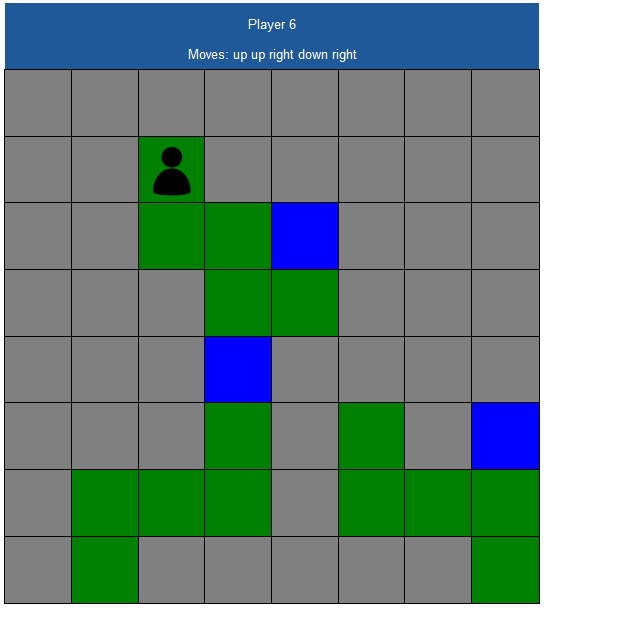
\includegraphics[scale=0.5]{Team1.png}\\
Late game screen in a game with two teams of three players each
\end{center}

\begin{center}
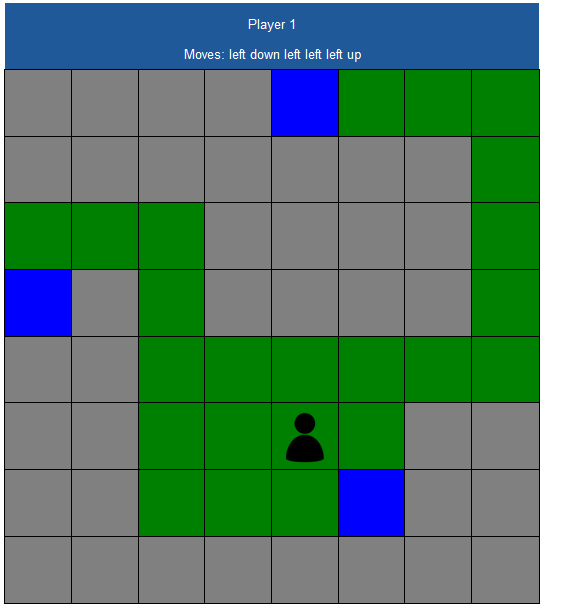
\includegraphics[scale=0.5]{Team2.png}\\
Late game screen of a game between two players
\end{center}

\noindent One can see the different patches of tiles in a team game, this is because there are different players playing and so every player on the team is able to observe the tiles, unlike a game not in cooperative mode where all the tiles are those which a player has visited on already.\\

\newpage 
\section{Code Coverage}
\subsection{Basic Version of the Game}

After finishing our development and testing of the basic version of the game, our code coverage statistics taken from Jenkins were as follows.

\begin{center}
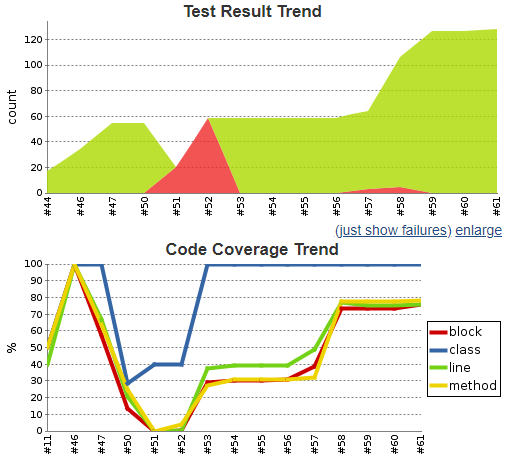
\includegraphics[scale = 0.75]{Figure4.png}\\
\end{center}

\noindent Using the built in code coverage plug-in in IntelliJ, we were able to take note of which methods were not covered by our unit tests to ensure that each method which was not covered was left this way with good reason. The methods which were not tested are all in the \textbf{Game} class. An explanation of why these methods were not covered is given below.

\begin{itemize}

     \item \textit{Main} method:\\
     This method simply calls other methods to initialise the game and run the main game loop. Each of 	  	 these methods are tested individually
     
     \item \textit{startGame} method:\\
     Like the Main method, this method calls other methods to initialise the map and players. Each of    	 these methods are tested individually
     
     \item \textit{getPlayerNum} method:\\
     This method simply receives a user input and passes it to the \textit{validatePlayerNum} method 	     	 which ensures that the input is an integer within the allowed range (2-8). All the testing for  	 	 this is therefore done in the \textit{validatePlayerNum} method.
     
     \item \textit{getMapSize} method:\\
     This method simply receives a user input and passes it to the \textit{validateMapSize} method 	      	 which ensures that the input is an integer within the allowed range (5-50 depending on the number  	     of players). All the testing for this is therefore done in the \textit{validateMapSize} method.
     
     \item \textit{directionsLoop} method:\\
     This method is a loop which asks each player for the direction they would like to move in and   	 	 then checks that this move is allowed with the \textit{checkOutOfBounds} and  	  	 					     \textit{validateDirectionInput} methods. If it is then the \textit{move} method in the 	 	  	 	 \textbf{Player} class is called upon to execute the desired move. The \textit{checkOutOfBounds}              	 and \textit{validateDirection} input methods are both tested to make sure that only a valid 	 	 	 direction is accepted and the \textit{move} method in the \textbf{Player} class is also tested to 	    	 make sure every move case can be properly handled by the program. Therefore, there is no need to 		     test the \textit{directionsLoop} method.
     
     \item \textit{endGame} method:\\
     This method receives a character from the \textit{getExitChar} method. If this character is 'e' 		     then the map html files are deleted using the \textit{deleteHtmlFiles} method and the program is 		     exited. The \textit{getExitChar} method is tested individually using the 			 	 				 	 \textit{validateExitChar} method to ensure that only 'e' causes the program to exit. The 				 	 \textit{deleteHtmlFiles} method is also tested individually to ensure that the files are deleted 		 	 correctly every time. There is therefore no need to test the \textit{endGame} method.
     
     \item \textit{getExitChar} method:\\
     This method receives a character user input from the user which is validated in the 					 	 \textit{validateExitChar} method. If this input is 'e' then it is returned to the 						 	 \textit{endGame} method which will delete the map html files and exit the program. Since it is 		 	 tested in the \textit{validateExitChar} method, \textit{getExitChar} does not need to be tested.
     
\end{itemize}
\newpage

\subsection{The Game After Enhancements}

After we finished adding and testing the required enhancements to the game, our code coverage statistics taken from Jenkins were as follows.

\begin{center}
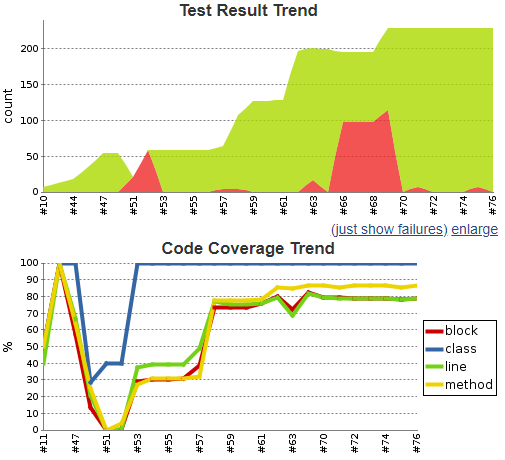
\includegraphics[scale = 0.75]{Figure5.png}\\
\end{center}

\noindent Again, using the built in code coverage plug-in in IntelliJ, we took note of which methods were not covered by our unit tests to ensure that each method which was not covered was left this way with good reason. The methods which were not tested in the basic version of the game are still not tested in this version for the same reasons and will therefore not be explained again. An explanation of why some of the new methods were not covered is given below.

\renewcommand\labelitemii{$\triangleright$}
\begin{itemize}
    \item \textbf{Game} class:\\
    \vspace{-5mm}
    \begin{itemize}
  		\item \textit{getTeamNum} method:\\
  		This method simply receives a user input and passes it to the \textit{validateTeamNum} method 	     		which ensures that the input is an integer within the allowed range (between 2 and the amount of 		players). All the testing for this is therefore done in the \textit{validateTeamNum} method.
  		
  		\item \textit{getMapType} method:\\
  		This method simply receives a user input and passes it to the \textit{validateMapType} method 	     		which ensures that the input is a string which is either "safe" or "hazardous". All the testing 			for this is therefore done in the \textit{validateMapType} method.
  	\end{itemize}
  	\newpage
	
	\item \textbf{MapCreator} class:\\
	\vspace{-5mm}
	\begin{itemize}
		\item \textit{create} method:\\
		This method is overridden in the \textbf{SafeMapCreator} and \textbf{HazardousMapCreator} 					classes and each of these override methods are tested individually. There is therefore no need 				to test this method.
	\end{itemize}
\end{itemize}
\newpage 

\section{Instructions to Run The Game}

\begin{enumerate}
	\item Download and extract the project from\\
	\url{https://github.com/martin-and-mikhail/CPS2002_MartinMikhail}\\
	Please note that the "Part1", "Part2" and "Part3" tags can be used to view the 
	
	\item Compile and run \textbf{Game.java} to run the game or run the \textbf{Game} class from an IDE
	
	\item Configure the game by choosing the amount of players, amount of teams, and the size and type 		 	of map. Each player will then be shown which team they are on. An example of this is shown below.
	
	\begin{center}
	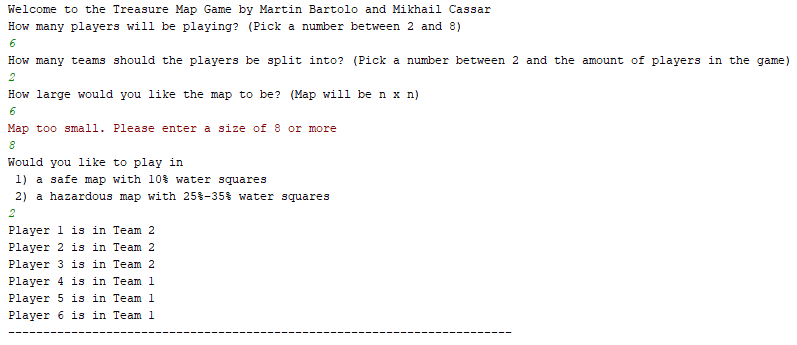
\includegraphics[scale=0.65]{Figure6.png}\\
	\end{center}
	
	\item Open up the map.html file in a browser. Each player will be at a random starting position at 			this point in the game.
	
	\item The game will now start. In each round, each player will be prompted to enter their desired 			direction of movement. This can be done by entering u, d, l or r and then pressing enter to confirm 		the direction. If the player lands on a grass tile, they and their team members will have this tile 		changed to green on their map. If the player lands on a water tile, they will be notified and will 			be moved back to their starting position. This tile will also be marked on the player and their team 	mates' maps. If the player lands on the treasure tile then they will be marked as one of the game's 		winners, along with anyone else who lands on the treasure in the round, at the end of the round. 			Please note that the map is updated before each player must input a direction. Make sure to refresh 		the browser after every move is made.
\end{enumerate}

\end{document}
